\newsection
\section{Graph theory}
\begin{definition}[]{Graphs: Directed and Undirected}
    A \textbf{graph} $G = (V, E)$ consists of:
    \begin{itemize}
        \item A set of \textbf{vertices} (or nodes) $V$, and
        \item A set of \textbf{edges} $E$, representing connections between pairs of vertices.
    \end{itemize}
    Graphs can be classified into:
    \begin{itemize}
        \item \textbf{Undirected Graphs:} Edges have no direction, represented as unordered pairs $\{u, v\}$.
        \item \textbf{Directed Graphs (Digraphs):} Edges have a direction, represented as ordered pairs $(u, v)$.
    \end{itemize}
\end{definition}

\begin{terms}[]{Graph Theory}
    \begin{itemize}
        \item \textbf{Adjacent (Neighbors):} Two vertices $u$ and $v$ are adjacent if there is an edge between them.
        \item \textbf{Degree:}
              \begin{itemize}
                  \item \textbf{Undirected Graph:} The degree of a vertex $v$ is the number of edges incident to it.
                  \item \textbf{Directed Graph:}
                        \begin{itemize}
                            \item \textbf{In-Degree:} Number of incoming edges to $v$.
                            \item \textbf{Out-Degree:} Number of outgoing edges from $v$.
                        \end{itemize}
              \end{itemize}
        \item \textbf{Path:} A sequence of vertices where each adjacent pair is connected by an edge.
              \begin{itemize}
                  \item \textbf{Simple Path:} A path with no repeated vertices.
                  \item \textbf{Cycle:} A path that starts and ends at the same vertex.
              \end{itemize}
        \item \textbf{Connected Graph:} A graph where there is a path between any two vertices.
              \begin{itemize}
                  \item \textbf{Strongly Connected:} In a directed graph, every vertex is reachable from every other vertex.
                  \item \textbf{Weakly Connected:} A directed graph becomes connected if the direction of edges is ignored.
              \end{itemize}
        \item \textbf{Subgraph:} A graph formed from a subset of vertices and edges of the original graph.
        \item \textbf{Complete Graph:} A graph in which every pair of vertices is connected by an edge.
        \item \textbf{Weighted Graph:} A graph where each edge has an associated weight or cost.
        \item \textbf{Multigraph:} A graph that may have multiple edges (parallel edges) between the same pair of vertices.
        \item \textbf{Self-Loop:} An edge that connects a vertex to itself.
        \item \textbf{Bipartite Graph:} A graph whose vertices can be divided into two disjoint sets such that every edge connects a vertex in one set to a vertex in the other set.
        \item \textbf{Tree:} A graph is a tree if it is connected and has no cycles (sufficient condition), a tree has $n - 1$ edges for $n$ vertices (necessary condition).
        \item \textbf{Reachability:} A vertex $u$ is called \textit{reachable} from $v$, if there exists a walk or path with endpoints $u$ and $v$.
    \end{itemize}
\end{terms}

\begin{example}[]{Directed and Undirected Graphs}
    \begin{center}
        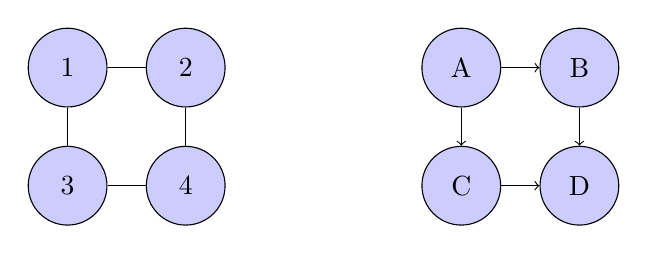
\begin{tikzpicture}[node distance=1.5cm, main/.style={circle, draw, fill=blue!20, minimum size=10mm, inner sep=0pt}]
            % Undirected graph
            \node[main] (1) {1};
            \node[main] (2) [right of=1] {2};
            \node[main] (3) [below of=1] {3};
            \node[main] (4) [below of=2] {4};
            \draw (1) -- (2);
            \draw (1) -- (3);
            \draw (3) -- (4);
            \draw (2) -- (4);

            % Directed graph
            \node[main] (5) [right of=2, xshift=2cm] {A};
            \node[main] (6) [right of=5] {B};
            \node[main] (7) [below of=5] {C};
            \node[main] (8) [below of=6] {D};
            \draw[->] (5) -- (6);
            \draw[->] (5) -- (7);
            \draw[->] (7) -- (8);
            \draw[->] (6) -- (8);
        \end{tikzpicture}
    \end{center}
\end{example}
